\def\doctitle{Demo: Kelvin Water Dropper}
\def\docsubtitle{Prove electrostatic feedback without making a spark}
\def\docstrap{adult-built apparatus; measured evidence; stop early}
\def\materialslist{\item Adult-built paired drip apparatus in a deep spill tray
\item Two collector cans, two induction rings, and insulated cross-coupling
\item Two adjustable plastic water lines with matched nozzles
\item Low-capacitance electroscope with a fixed millimetre scale
\item Stopwatch, ruler, two measuring cups, paper towels
\item Designed high-resistance discharge lead, used only after flow stops}
\def\prediction{Before water starts, choose one: will both electroscope leaves
remain still, move together, or separate? What visible change would count as
evidence for charge separation if sparks are forbidden? Predict which matters
more: the total water delivered, or whether each stream breaks into droplets
inside its induction ring.}

\def\diagram{%
\begin{center}
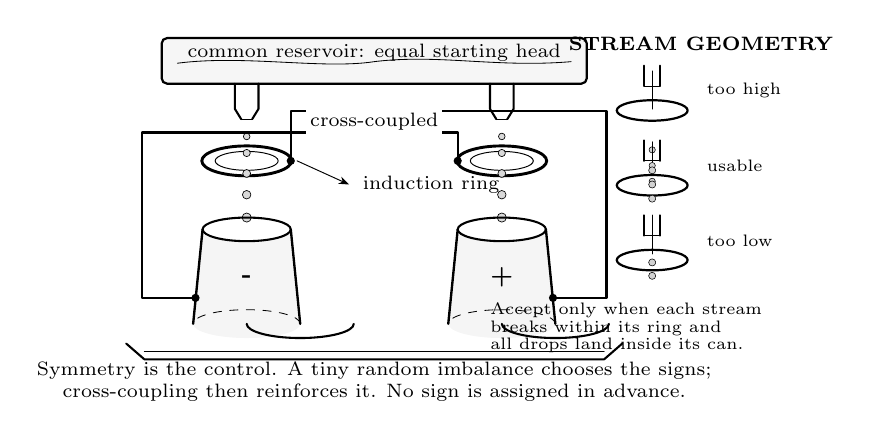
\begin{tikzpicture}[x=1cm,y=1cm,line cap=round,line join=round,
  note/.style={font=\scriptsize,align=left},
  tinylabel/.style={font=\fontsize{5.6}{6.4}\selectfont,align=center},
  wire/.style={line width=.75pt},
  leader/.style={line width=.35pt,-{Stealth[length=1.3mm]}}]
  % Reservoir and paired nozzles.
  \path[fill=gray!7,rounded corners=2pt] (-2.70,1.80) rectangle (2.70,2.38);
  \draw[line width=.8pt,rounded corners=2pt] (-2.70,1.80) rectangle (2.70,2.38);
  \draw[line width=.3pt] (-2.50,2.06)
    .. controls (-1.65,2.17) and (-.65,1.98) .. (0,2.08)
    .. controls (.82,2.18) and (1.55,2.00) .. (2.50,2.08);
  \node[font=\scriptsize] at (0,2.20) {common reservoir: equal starting head};
  \foreach \x in {-1.62,1.62}{
    \draw[line width=.75pt] (\x-.15,1.80)--(\x-.15,1.48)--(\x-.07,1.35);
    \draw[line width=.75pt] (\x+.15,1.80)--(\x+.15,1.48)--(\x+.07,1.35);
    \draw[line width=.35pt] (\x-.07,1.35)--(\x+.07,1.35);
    \draw[line width=1.05pt] (\x,.82) ellipse (.57 and .19);
    \draw[line width=.35pt] (\x,.82) ellipse (.40 and .12);
    \foreach \y/\r in {1.13/.042,.92/.046,.66/.050,.39/.054,.10/.058}
      \path[fill=gray!30,draw=black,line width=.24pt] (\x,\y) circle (\r);
  }
  % Collector cans.
  \foreach \x/\sgn in {-1.62/-,1.62/+}{
    \path[fill=gray!8] (\x-.68,-1.25)--(\x-.56,-.05)
      arc[start angle=180,end angle=360,x radius=.56,y radius=.15]
      --(\x+.68,-1.25) arc[start angle=0,end angle=-180,x radius=.68,y radius=.18]--cycle;
    \draw[line width=.85pt] (\x-.68,-1.25)--(\x-.56,-.05);
    \draw[line width=.85pt] (\x+.68,-1.25)--(\x+.56,-.05);
    \draw[line width=.75pt] (\x,-.05) ellipse (.56 and .15);
    \draw[line width=.75pt] (\x,-1.25) arc[start angle=180,end angle=360,x radius=.68,y radius=.18];
    \draw[line width=.3pt,dashed] (\x+.68,-1.25) arc[start angle=0,end angle=180,x radius=.68,y radius=.18];
    \node[font=\small\bfseries] at (\x,-.66) {\sgn};
  }
  % Cross-coupling.
  \draw[wire] (-2.27,-.92)--(-2.95,-.92)--(-2.95,1.18)--(1.06,1.18)--(1.06,.82);
  \draw[wire] (2.27,-.92)--(2.95,-.92)--(2.95,1.45)--(-1.06,1.45)--(-1.06,.82);
  \foreach \p in {(-2.27,-.92),(2.27,-.92),(1.06,.82),(-1.06,.82)}
    \fill \p circle (.052);
  \draw[line width=.75pt] (-3.15,-1.50)--(-2.92,-1.70)--(2.92,-1.70)--(3.15,-1.50);
  \draw[line width=.35pt] (-2.92,-1.60)--(2.92,-1.60);
  \node[note,fill=white,inner sep=1.5pt] at (0,1.32) {cross-coupled};
  \draw[leader] (-.98,.82)--(-.32,.52);
  \node[note,anchor=west] at (-.27,.52) {induction ring};
  \node[note,align=center] at (0,-1.98)
    {Symmetry is the control. A tiny random imbalance chooses the signs;\\
     cross-coupling then reinforces it. No sign is assigned in advance.};

  % Three observable stream states.
  \begin{scope}[shift={(4.15,.96)}]
    \node[font=\scriptsize\bfseries] at (0,1.35) {STREAM GEOMETRY};
    \foreach \yy/\lab in {.75/{too high},-.20/{usable},-1.15/{too low}}{
      \draw[line width=.65pt] (-.72,\yy+.32)--(-.72,\yy+.06);
      \draw[line width=.65pt] (-.52,\yy+.32)--(-.52,\yy+.06);
      \draw[line width=.3pt] (-.72,\yy+.06)--(-.52,\yy+.06);
      \draw[line width=.8pt] (-.62,\yy-.25) ellipse (.45 and .13);
      \node[tinylabel,anchor=west] at (-.05,\yy) {\lab};
    }
    % Continuous through ring.
    \draw[line width=.5pt] (-.62,1.00)--(-.62,.52);
    \foreach \y in {.00,-.20,-.40}
      \fill[gray!35,draw=black,line width=.2pt] (-.62,\y) circle (.04);
    % Break point centred in ring.
    \draw[line width=.5pt] (-.62,.10)--(-.62,-.15);
    \foreach \y in {-.26,-.44,-.62}
      \fill[gray!35,draw=black,line width=.2pt] (-.62,\y) circle (.045);
    % Break below ring.
    \draw[line width=.5pt] (-.62,-.83)--(-.62,-1.32);
    \foreach \y in {-1.43,-1.60}
      \fill[gray!35,draw=black,line width=.2pt] (-.62,\y) circle (.045);
    \node[tinylabel,anchor=north,align=left] at (-.95,-1.82)
      {Accept only when each stream\\breaks within its ring and\\all drops land inside its can.};
  \end{scope}
\end{tikzpicture}
\end{center}}

\def\procedure{%
\subsection{Adult preflight --- water off}
The learner observes from the marked boundary and does not touch the apparatus.
The adult confirms all six items before proceeding:
\begin{enumerate}
\item Tray, frame, reservoir, cans, and rings are stable; the floor and nearby
surfaces are dry. There are no exposed sharp edges.
\item The two cans are well separated, each ring is centred over its own can,
and no loose wire can swing toward another conductor.
\item Each collector is connected only to the \emph{opposite} ring. Trace both
paths aloud. Same-side coupling is a wiring error.
\item The electroscope begins at zero and its scale can be read without anyone
approaching the apparatus.
\item The intended high-resistance discharge lead is present, intact, and
parked. It is not a hand-held improvised wire.
\item Stop immediately for a snap, visible spark, hair movement, tingling,
unstable support, escaping water, or an electroscope reading above the chosen
conservative stop mark.
\end{enumerate}

\subsection{Establish a hydraulic control}
Ground and discharge the apparatus by its designed method. Run water for
10 seconds with charge unable to accumulate. Catch each stream separately,
count its drops from slow-motion video or direct observation, and measure its
volume. Adjust only the water controls until both streams break inside their
rings, land centrally, and agree closely. Record the evidence; do not call
``looks equal'' a measurement.

\begin{center}
\small
\begin{tabular}{@{}lcccc@{}}
\toprule
Run & left drops/10 s & right drops/10 s & left mL/10 s & right mL/10 s\\
\midrule
hydraulic control & \rule{1.5cm}{.3pt} & \rule{1.5cm}{.3pt}
 & \rule{1.4cm}{.3pt} & \rule{1.4cm}{.3pt}\\
\bottomrule
\end{tabular}
\end{center}

\subsection{Observe charge separation without discharge}
Stop the water. Discharge through the intended high-resistance path, verify
zero, then park the lead. Start the matched drips and the stopwatch together.
From the boundary, read electroscope deflection against the fixed scale every
five seconds. Stop at 20 seconds or at the preselected stop mark, whichever
comes first. Repeat from a verified zero. A repeatable rise is evidence; one
twitch is not.

\begin{center}
\small
\begin{tabular}{@{}lccccc@{}}
\toprule
Run & 0 s & 5 s & 10 s & 15 s & 20 s\\
\midrule
deflection, mm & \rule{1.0cm}{.3pt} & \rule{1.0cm}{.3pt}
 & \rule{1.0cm}{.3pt} & \rule{1.0cm}{.3pt} & \rule{1.0cm}{.3pt}\\
repeat, mm & \rule{1.0cm}{.3pt} & \rule{1.0cm}{.3pt}
 & \rule{1.0cm}{.3pt} & \rule{1.0cm}{.3pt} & \rule{1.0cm}{.3pt}\\
\bottomrule
\end{tabular}
\end{center}

\subsection{Return to a proved-safe state}
Water off first. Wait for every drop to land. Apply the designed discharge
path without touching either collector, hold it as specified for the apparatus,
and verify the electroscope returns to zero. Only then may the adult approach.
Dry the tray and floor before any adjustment.}

\def\explanation{The hydraulic control shows that both sides began with similar
water flow. During the isolated runs, a growing electroscope deflection shows
that charge accumulated even though no battery was connected and no spark was
allowed. A minute accidental imbalance polarizes the falling water. Each
charged collector biases the opposite stream through its induction ring, so
the imbalance reinforces itself. The falling water supplies the energy; the
cross-coupling supplies positive feedback.

\medskip
\noindent\textbf{Interrogate the evidence.}
Did both repeated runs rise from zero? Was the direction consistent, or did the
apparatus choose either sign? Could unequal drip rates explain the result?
Which observation distinguishes feedback from a single charged object:
continued growth, reversal after swapping a connection, or one initial jump?}

\def\extension{%
\textbf{Change only drip rate.} After discharge and a verified zero, make both
streams slightly slower while preserving their break points inside the rings.
Repeat the same 20-second table. Compare the slope in millimetres per five
seconds, not the maximum reading and never spark length.

\medskip
\noindent\textbf{If the trace stays flat, troubleshoot conservatively.}
\par\smallskip
\begin{tabularx}{\linewidth}{@{}p{.28\linewidth}X@{}}
\toprule
Observation & Water-off correction after discharge and zero verification\\
\midrule
Both traces remain at zero & Trace opposite-side coupling; check that the
electroscope responds to its approved test; dry insulators and tray.\\
One stream is continuous & Reduce flow until breakup occurs inside its ring;
do not move a live ring.\\
Drops hit a ring or miss a can & Re-centre with water off; confirm supports
cannot drift before restarting.\\
One run rises, the repeat does not & Restore the measured hydraulic control,
dry all surfaces, and repeat from a verified zero.\\
Reading jumps or nears stop mark & Stop water immediately, discharge by the
designed path, and increase separation before any further run.\\
\bottomrule
\end{tabularx}

\medskip
\begin{center}
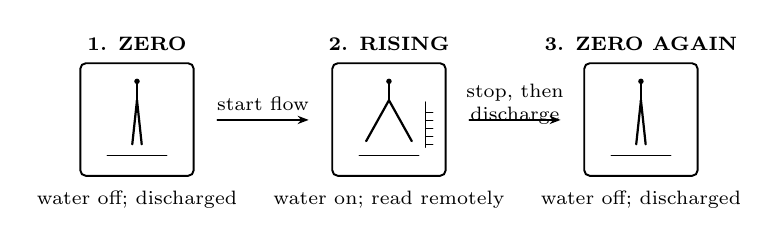
\begin{tikzpicture}[x=1cm,y=1cm,line cap=round,
  state/.style={font=\scriptsize\bfseries},
  sub/.style={font=\scriptsize,align=center}]
  \foreach \x/\title/\caption in {0/{1. ZERO}/{water off; discharged},
    3.2/{2. RISING}/{water on; read remotely},
    6.4/{3. ZERO AGAIN}/{water off; discharged}}{
    \draw[line width=.7pt,rounded corners=2pt] (\x-.72,-.48) rectangle (\x+.72,.95);
    \draw[line width=.55pt] (\x,.72)--(\x,.48);
    \fill (\x,.72) circle (.035);
    \draw[line width=.35pt] (\x-.38,-.22)--(\x+.38,-.22);
    \node[state] at (\x,1.20) {\title};
    \node[sub] at (\x,-.78) {\caption};
  }
  % Closed leaves at both proved-zero states.
  \draw[line width=.8pt] (0,.48)--(-.06,-.08);
  \draw[line width=.8pt] (0,.48)--(.06,-.08);
  \draw[line width=.8pt] (6.4,.48)--(6.34,-.08);
  \draw[line width=.8pt] (6.4,.48)--(6.46,-.08);
  % Deflected leaves and a fixed millimetre scale.
  \draw[line width=.8pt] (3.2,.48)--(2.91,-.04);
  \draw[line width=.8pt] (3.2,.48)--(3.49,-.04);
  \draw[line width=.35pt] (3.67,-.12)--(3.67,.46);
  \foreach \y in {-.08,.02,...,.42} \draw[line width=.25pt] (3.67,\y)--(3.76,\y);
  \draw[-{Stealth[length=1.4mm]},line width=.55pt] (1.02,.23)--(2.18,.23);
  \draw[-{Stealth[length=1.4mm]},line width=.55pt] (4.22,.23)--(5.38,.23);
  \node[sub] at (1.60,.43) {start flow};
  \node[sub] at (4.80,.43) {stop, then\\discharge};
\end{tikzpicture}
\end{center}

\noindent The evidence is a complete state change, not merely a large reading:
a verified neutral start, gradual deflection while drops fall, and a verified
neutral finish after the prescribed shutdown.

\medskip
\noindent\textbf{Final proof.} Accept the demonstration only if two isolated
runs begin at zero, show a gradual measurable rise before the stop mark, make
no spark or snap, keep every drop inside the collectors, and end at verified
zero after high-resistance discharge. Otherwise record ``not demonstrated''
and stop.}
% Telos shared preamble.
%
% Every Telos publication is designed to be printed on a home laser printer,
% one sheet at a time, and carried into a boat or a garage. Two constraints
% follow from that and govern everything below:
%
%   1. Pure monochrome. No value is ever a hue. Emphasis is carried by rule
%      weight, fill, and type, never by color, so a grayscale or black-only
%      printer loses nothing.
%   2. Card density. A "one-pager" is a hard contract: the leaf must fit on a
%      single side of US Letter. The layout is therefore tight by default and
%      the environments below are sized to leave room for a plate.

\documentclass[10pt,letterpaper]{article}

\usepackage[margin=0.55in,includefoot,footskip=0.24in]{geometry}
\usepackage[T1]{fontenc}
\usepackage[utf8]{inputenc}
\usepackage{lmodern}
\usepackage{microtype}
\usepackage{array}
\usepackage{booktabs}
\usepackage{longtable}
\usepackage{tabularx}
\usepackage{enumitem}
\usepackage{needspace}
\usepackage{multicol}
\usepackage{ragged2e}
\usepackage{graphicx}
\usepackage{wrapfig}
\usepackage{xcolor}
\usepackage{fancyhdr}
\usepackage{titlesec}
\usepackage{hyperref}
\usepackage[most]{tcolorbox}
\usepackage{tikz}
\usetikzlibrary{arrows.meta,calc,positioning,shapes.geometric,decorations.pathmorphing,patterns,fadings}

% Semantic names are kept so a document reads intelligibly, but every value is
% black, white, or a neutral gray that survives a black-only print driver.
\definecolor{telosink}{gray}{0}
\definecolor{telospaper}{gray}{1}
\definecolor{telosrule}{gray}{0.35}
\definecolor{telosfill}{gray}{0.90}
\definecolor{telosdeep}{gray}{0.72}
\definecolor{telosmute}{gray}{0.45}

\hypersetup{hidelinks,pdfborder={0 0 0}}

% Keep an unchanged source byte-reproducible across rebuilds: no build-clock
% creation date and no random trailer ID.
\pdfinfoomitdate=1
\pdftrailerid{}

\setlength{\parindent}{0pt}
\setlength{\parskip}{0.42em}
\setlength{\tabcolsep}{4pt}
\setlength{\columnsep}{1.1em}
\renewcommand{\arraystretch}{1.18}
\setlist[itemize]{leftmargin=1.15em,itemsep=0.12em,topsep=0.2em,parsep=0pt}
\setlist[enumerate]{leftmargin=1.5em,itemsep=0.18em,topsep=0.2em,parsep=0pt}
\setlist[description]{leftmargin=0pt,itemsep=0.16em,topsep=0.2em,parsep=0pt,
  font=\normalfont\bfseries}

% ---------------------------------------------------------------------------
% Document identity. Each leaf declares these before \begin{document} so the
% running head, the colophon, and the PDF metadata all agree.
% ---------------------------------------------------------------------------
\newcommand{\TelosProject}{Telos}
\newcommand{\TelosDocTitle}{}
\newcommand{\TelosDocSubtitle}{}
\newcommand{\TelosRevision}{}

\newcommand{\telosmeta}[4]{%
  \renewcommand{\TelosProject}{#1}%
  \renewcommand{\TelosDocTitle}{#2}%
  \renewcommand{\TelosDocSubtitle}{#3}%
  \renewcommand{\TelosRevision}{#4}%
  \hypersetup{pdftitle={#2},pdfsubject={#3; version #4},
    pdfkeywords={Telos, version #4},pdfauthor={Telos}}%
}

\pagestyle{fancy}
\fancyhf{}
\renewcommand{\headrulewidth}{0pt}
\renewcommand{\footrulewidth}{0.4pt}
\fancyfoot[L]{\footnotesize\textsc{\TelosProject}}
\fancyfoot[C]{\footnotesize\TelosDocTitle}
\fancyfoot[R]{\footnotesize\thepage}

% The first page of a one-pager carries the masthead instead of a running foot,
% so its footer is the compact provenance line.
\fancypagestyle{telosfirst}{%
  \fancyhf{}%
  \renewcommand{\headrulewidth}{0pt}%
  \renewcommand{\footrulewidth}{0.4pt}%
  \fancyfoot[L]{\footnotesize\textsc{\TelosProject}}%
  \fancyfoot[C]{\footnotesize\TelosRevision}%
  \fancyfoot[R]{\footnotesize\thepage}%
}

% ---------------------------------------------------------------------------
% Masthead. A heavy rule, the title, a light subtitle, a thin rule. The
% optional argument is a right-aligned tag (a species' scientific name, a
% lesson number) that sits on the title's baseline.
% ---------------------------------------------------------------------------
\newcommand{\telosmasthead}[1][]{%
  \thispagestyle{telosfirst}%
  \begingroup
  \setlength{\parskip}{0pt}%
  \noindent\rule{\linewidth}{1.6pt}\par
  \vspace{0.30em}
  \noindent
  \begin{minipage}[b]{0.66\linewidth}
    \raggedright{\LARGE\bfseries\TelosDocTitle}
  \end{minipage}%
  \hfill
  \begin{minipage}[b]{0.32\linewidth}
    \raggedleft{\small\itshape #1}
  \end{minipage}\par
  \vspace{0.18em}
  \noindent{\small\TelosDocSubtitle}\par
  \vspace{0.28em}
  \noindent\rule{\linewidth}{0.4pt}\par
  \endgroup
  \vspace{0.35em}
}

% ---------------------------------------------------------------------------
% Headings. Compact, small-caps, rule-anchored — a card has no room for the
% article class's default vertical air.
% ---------------------------------------------------------------------------
\titleformat{\section}{\normalfont\large\bfseries}{}{0pt}{}[\vspace{-0.55em}\rule{\linewidth}{0.4pt}]
\titlespacing*{\section}{0pt}{0.85em}{0.35em}
\titleformat{\subsection}{\normalfont\normalsize\bfseries}{}{0pt}{}
\titlespacing*{\subsection}{0pt}{0.6em}{0.2em}
\titleformat{\subsubsection}{\normalfont\small\bfseries\scshape}{}{0pt}{}
\titlespacing*{\subsubsection}{0pt}{0.45em}{0.12em}

% A short run-in heading for card interiors that must not consume a full line.
\newcommand{\telosrubric}[1]{\textbf{#1}\enspace}

% Cross-reference helper. Every Telos project is a set of loose printed sheets,
% so a reference names the sheet rather than a page number.
\newcommand{\sheetref}[1]{\textit{see the \textbf{#1} sheet}}

% Which decision, ADR or sheet governs the paragraph you are reading. A reader
% who disagrees with an instruction should be able to find the reasoning behind
% it rather than having to take it on trust.
\newcommand{\governedby}[1]{{\footnotesize\textsc{governed by #1}}}

% ---------------------------------------------------------------------------
% Quantities. siunitx is not in this TeX Live split, and the guides need only a
% fixed thin space and upright units, so define that directly rather than take
% a package dependency the documented install would not satisfy.
%   \qty{9}{kV}  ->  9 kV        \unitof{kV}  ->  kV
% ---------------------------------------------------------------------------
\newcommand{\unitof}[1]{\ensuremath{\mathrm{#1}}}
\newcommand{\qty}[2]{#1\,\unitof{#2}}
\newcommand{\numrange}[2]{#1\,--\,#2}
\newcommand{\qtyrange}[3]{#1\,--\,#2\,\unitof{#3}}
% Inches and feet appear constantly in the fishing guide; keep one spelling.
\newcommand{\inch}[1]{#1\,in}
\newcommand{\feet}[1]{#1\,ft}

% ---------------------------------------------------------------------------
% Cards and boxes.
% ---------------------------------------------------------------------------

% Titled card with a hairline frame. The default card for facts a reader looks
% up rather than reads through.
\newtcolorbox{teloscard}[1]{
  enhanced, breakable,
  colback=telospaper, colframe=telosink, colbacktitle=telospaper,
  coltitle=telosink,
  boxrule=0.5pt, sharp corners,
  left=6pt, right=6pt, top=4pt, bottom=4pt,
  toptitle=3pt, bottomtitle=3pt, titlerule=0.4pt,
  before skip=6pt, after skip=6pt,
  title={#1}, fonttitle=\small\bfseries
}

% Untitled left-ruled block: hierarchy without a redundant label.
\newtcolorbox{telosframe}{
  enhanced, breakable,
  colback=telospaper, frame hidden, boxrule=0pt, sharp corners,
  borderline west={1.3pt}{0pt}{telosink},
  left=8pt, right=2pt, top=3pt, bottom=3pt,
  before skip=6pt, after skip=6pt
}

% Filled emphasis panel — the "read this first" block. The 10% fill stays
% legible under a cheap laser toner curve and still reads as distinct.
\newtcolorbox{telospanel}[1]{
  enhanced, breakable,
  colback=telosfill, colframe=telosink, colbacktitle=telosfill,
  coltitle=telosink,
  boxrule=0.5pt, sharp corners,
  left=6pt, right=6pt, top=4pt, bottom=4pt,
  toptitle=3pt, bottomtitle=3pt, titlerule=0.4pt,
  before skip=6pt, after skip=6pt,
  title={#1}, fonttitle=\small\bfseries
}

% Hazard block. Deliberately the heaviest object on any page: a 1.4pt frame
% plus a solid title bar. Nothing else in Telos is allowed to look like this,
% so a reader skimming a lesson cannot mistake it for ordinary emphasis.
\newtcolorbox{teloshazard}[1]{
  enhanced, breakable,
  colback=telospaper, colframe=telosink,
  colbacktitle=telosink, coltitle=telospaper,
  boxrule=1.4pt, sharp corners,
  left=6pt, right=6pt, top=5pt, bottom=5pt,
  toptitle=3pt, bottomtitle=3pt,
  before skip=8pt, after skip=8pt,
  title={\MakeUppercase{#1}}, fonttitle=\small\bfseries
}

% A stop-and-check gate. Used before anything destructive, and before anything
% that would be expensive to discover later. Shared by every project that has
% a procedure someone could get hurt following carelessly.
\newtcolorbox{gate}[1]{
  enhanced, breakable,
  colback=telospaper, colframe=telosink,
  boxrule=1.0pt, sharp corners,
  left=6pt, right=6pt, top=4pt, bottom=4pt,
  toptitle=3pt, bottomtitle=3pt, titlerule=0.4pt,
  before skip=7pt, after skip=7pt,
  colbacktitle=telospaper, coltitle=telosink,
  title={\MakeUppercase{#1}}, fonttitle=\small\bfseries
}

% ---------------------------------------------------------------------------
% Rating dots. A five-step scale that prints identically in black-only: filled
% versus open circles, never a shaded bar.
% ---------------------------------------------------------------------------
\newcommand{\telosdot}{\tikz[baseline=-0.42ex]\fill[telosink] (0,0) circle (0.28ex);}
\newcommand{\telosopendot}{\tikz[baseline=-0.42ex]\draw[telosink,line width=0.28pt] (0,0) circle (0.28ex);}
\makeatletter
\newcounter{telos@rate}
\newcommand{\telosrating}[1]{%
  \begingroup
  \setcounter{telos@rate}{0}%
  \@whilenum\value{telos@rate}<#1\do{\telosdot\kern0.22em\stepcounter{telos@rate}}%
  \@whilenum\value{telos@rate}<5\do{\telosopendot\kern0.22em\stepcounter{telos@rate}}%
  \endgroup
}
\makeatother

% ---------------------------------------------------------------------------
% Tables.
%
% tabularx reads its body by scanning for a literal \end{tabularx}, so it can
% never be wrapped in a \newenvironment. Documents therefore open tabularx and
% longtable directly and take their house style from these column types and the
% booktabs rules. The one exception is the fact strip below, which is built on
% plain tabular precisely so it *can* be an environment.
% ---------------------------------------------------------------------------
\newcolumntype{L}{>{\raggedright\arraybackslash}X}
\newcolumntype{R}{>{\raggedleft\arraybackslash}X}
\newcolumntype{C}{>{\centering\arraybackslash}X}
\newcolumntype{B}{>{\bfseries\raggedright\arraybackslash}X}
\newcolumntype{N}{>{\raggedright\arraybackslash}p{0.16\linewidth}}

% Key/value fact strip. Two flush columns of short lookups; the label column is
% a fixed fraction so a stack of cards aligns across the whole guide.
\newenvironment{telosfacts}[1][0.24]
  {\begingroup\small
   \setlength{\parskip}{0pt}%
   \renewcommand{\arraystretch}{1.25}%
   \begin{tabular}{@{}>{\bfseries\raggedright\arraybackslash}p{\dimexpr#1\linewidth\relax}@{\hspace{0.7em}}>{\raggedright\arraybackslash}p{\dimexpr\linewidth-#1\linewidth-0.7em\relax}@{}}}
  {\end{tabular}\par\endgroup}
\newcommand{\telosfact}[2]{#1 & #2\\}

% ---------------------------------------------------------------------------
% Seasonal / diurnal activity bar.
%
% \telosseasonbar{4,3,2,1,1,2,3,3,4,5,4,3} draws a twelve-cell month strip
% where each value 0-5 is a fill height. Height, not gray value, carries the
% signal, so it is exact under any toner curve; the cell is outlined either way
% so an empty month is still visibly a month.
% ---------------------------------------------------------------------------
\newcommand{\telosseasonlabels}{J,F,M,A,M,J,J,A,S,O,N,D}
\newcommand{\telosseasonbar}[1]{%
  \begingroup
  \begin{tikzpicture}[x=1.25em,y=2.1ex,baseline=0pt]
    \foreach \v [count=\i from 0] in {#1} {
      \draw[telosrule,line width=0.3pt] (\i,0) rectangle (\i+0.86,5);
      \ifnum\v>0
        \fill[telosink] (\i,0) rectangle (\i+0.86,\v);
      \fi
    }
    \foreach \m [count=\i from 0] in \telosseasonlabels {
      \node[font=\tiny,anchor=north,inner sep=1.2pt] at (\i+0.43,-0.1) {\m};
    }
  \end{tikzpicture}%
  \endgroup
}

% Four-cell day-part strip: dawn, midday, dusk, night.
\newcommand{\telosdaylabels}{Dawn,Mid,Dusk,Night}
\newcommand{\telosdaybar}[1]{%
  \begingroup
  \begin{tikzpicture}[x=2.9em,y=2.1ex,baseline=0pt]
    \foreach \v [count=\i from 0] in {#1} {
      \draw[telosrule,line width=0.3pt] (\i,0) rectangle (\i+0.92,5);
      \ifnum\v>0
        \fill[telosink] (\i,0) rectangle (\i+0.92,\v);
      \fi
    }
    \foreach \m [count=\i from 0] in \telosdaylabels {
      \node[font=\tiny,anchor=north,inner sep=1.2pt] at (\i+0.46,-0.1) {\m};
    }
  \end{tikzpicture}%
  \endgroup
}

% A bar needs vertical room for its labels when it sits in a fact strip.
\newcommand{\telosbarrow}[1]{\rule{0pt}{4.2ex}#1\rule[-1.6ex]{0pt}{1.6ex}}

% ---------------------------------------------------------------------------
% Plates. A species or apparatus illustration with a caption rule beneath it.
% \telosplate{width fraction}{file}{caption}
% ---------------------------------------------------------------------------
\newcommand{\telosplate}[3]{%
  \begingroup
  \centering
  \includegraphics[width=#1\linewidth]{#2}\par
  \vspace{0.15em}
  \begin{minipage}{#1\linewidth}
    \rule{\linewidth}{0.4pt}\par
    \vspace{0.1em}
    {\footnotesize #3\par}
  \end{minipage}\par
  \endgroup
  \vspace{0.3em}
}

% TikZ drawing conventions shared by every rig, knot, and circuit diagram.
\tikzset{
  telos line/.style={draw=telosink,line width=0.7pt},
  telos hair/.style={draw=telosink,line width=0.35pt},
  telos heavy/.style={draw=telosink,line width=1.2pt},
  telos node/.style={draw=telosink,fill=telospaper,align=center,inner sep=4pt,font=\small},
  telos emphasis/.style={draw=telosink,line width=1.2pt,fill=telospaper,align=center,
    inner sep=4pt,font=\small\bfseries},
  telos label/.style={font=\scriptsize,inner sep=1.5pt},
  telos arrow/.style={-{Stealth[length=1.8mm]},draw=telosink,line width=0.6pt},
  telos dim/.style={|<->|,draw=telosink,line width=0.35pt},
  telos water/.style={draw=telosrule,line width=0.4pt,decorate,
    decoration={snake,amplitude=0.4mm,segment length=3mm}},
}

% ---------------------------------------------------------------------------
% Lesson furniture
% ---------------------------------------------------------------------------

% \lessonhead{number}{time}{who does what}
\newcommand{\lessonhead}[3]{%
  \par\noindent
  \begin{minipage}{\linewidth}
    \rule{\linewidth}{0.4pt}\par
    \vspace{0.3em}
    {\small\textbf{Lesson #1}\quad$\cdot$\quad #2\quad$\cdot$\quad #3\par}
    \vspace{0.25em}
    \rule{\linewidth}{0.4pt}
  \end{minipage}\par
  \vspace{0.5em}}

% The materials list. Two columns of short lines; a lesson that needs a long
% shopping list is a lesson that has not been thought through.
\newenvironment{materials}
  {\begin{telospanel}{What you need}\begin{multicols}{2}
   \begin{itemize}[leftmargin=1em,itemsep=0.05em,topsep=0pt]}
  {\end{itemize}\end{multicols}\end{telospanel}}

% The four rubrics every lesson carries, in the same order every time:
% what you are about to see, what to do, what it means, and what to ask.
\newcommand{\lessonsection}[1]{\section*{#1}\vspace{-0.35em}\rule{\linewidth}{0.4pt}\vspace{0.2em}}

% A prediction box. The point of the curriculum is that they commit to an
% answer before the demonstration, not after.
\newtcolorbox{predict}{
  enhanced, breakable,
  colback=telospaper, colframe=telosink,
  boxrule=0.5pt, sharp corners,
  left=6pt, right=6pt, top=4pt, bottom=4pt,
  before skip=6pt, after skip=6pt,
  borderline west={2.2pt}{0pt}{telosink},
  title={\small\bfseries Predict first}, fonttitle=\small\bfseries,
  colbacktitle=telospaper, coltitle=telosink,
  toptitle=3pt, bottomtitle=3pt, titlerule=0.4pt,
}

% ---------------------------------------------------------------------------
% Colophon. Rendered once, at the end of the last page, in the recovered footer
% area so it never creates a page of its own.
% ---------------------------------------------------------------------------
\newif\ifTelosColophonRendered
\newcommand{\TelosColophonExtra}{}
\newcommand{\TelosColophon}{%
  \ifTelosColophonRendered\else
  \global\TelosColophonRenderedtrue
  \par
  \enlargethispage{0.5in}%
  \vspace{0.3em}%
  \begingroup
  \setlength{\parskip}{0pt}%
  \begin{minipage}{\linewidth}
  \rule{\linewidth}{0.35pt}\par
  \vspace{0.3em}%
  \fontsize{7}{8.2}\selectfont
  \textbf{Telos.} \TelosProject{} — \TelosDocTitle. Revised \TelosRevision.
  \TelosColophonExtra{}
  Project-created text and diagrams are licensed \href{https://creativecommons.org/licenses/by/4.0/}{CC BY 4.0}.
  Incorporated public-domain artwork remains public domain and is credited on
  the plate it appears with. See \texttt{LICENSE} and \texttt{CREDITS.md} in the
  source. Nothing here is professional advice; verify current regulations and
  follow the stated safety procedure.
  \end{minipage}
  \endgroup
  \fi
}
\AtEndDocument{\TelosColophon}

\newcommand{\editiontag}{ChatGPT edition}
\newcommand{\boundary}{\textbf{Learner boundary:} isolated battery power only,
12 V DC maximum. No outlets, mains leads, opened appliances, large battery
packs, charged power capacitors, ignition coils, sparks, or exposed high
voltage. An adult facilitator is not thereby an electrically qualified person.}
\newenvironment{recordbox}{\begin{teloscard}{Evidence record}\small
\begin{tabularx}{\linewidth}{@{}p{.19\linewidth}L@{}}
Prediction & \rule{.95\linewidth}{.3pt}\\[1.1em]
One change & \rule{.95\linewidth}{.3pt}\\[1.1em]
Observation & \rule{.95\linewidth}{.3pt}\\[1.1em]
Claim + because & \rule{.95\linewidth}{.3pt}
\end{tabularx}}{\end{teloscard}}
\newcommand{\sourcefoot}{\par\smallskip{\footnotesize Physics and safety basis:
NIST SI/CODATA; OSHA 29 CFR 1910.333 and OSHA 3075; DOE Electrical Science
handbooks; HyperPhysics (Georgia State University); University of Colorado
PhET teacher resources. Full citations and scope notes are recorded in the
provider-neutral electricity research library.}}
\newcommand{\rolecard}{\begin{telospanel}{Stop line and roles}\boundary\par
\smallskip The learner predicts, assembles only the pictured battery circuit,
and records. The adult inspects parts, controls power, and stops heat, odor,
damage, pain, or unexpected behavior. Work outside this boundary belongs only
to a person qualified for that work.\end{telospanel}}
\newcommand{\circuitdiagram}{\begin{center}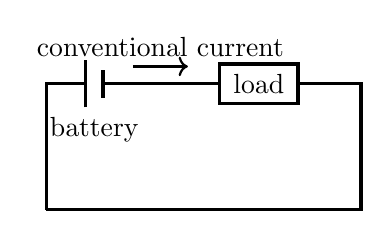
\begin{tikzpicture}[x=1cm,y=1cm]
\draw[very thick] (0,0)--(0,1.6)--(.5,1.6);
\draw[very thick] (.5,1.3)--(.5,1.9); \draw[very thick] (.72,1.42)--(.72,1.78);
\node[below] at (.61,1.3){battery};
\draw[very thick] (.72,1.6)--(2.2,1.6);
\draw[very thick] (2.2,1.35) rectangle (3.2,1.85);
\node at (2.7,1.6){load};
\draw[very thick] (3.2,1.6)--(4,1.6)--(4,0)--(0,0);
\draw[->,thick] (1.1,1.82)--(1.8,1.82) node[midway,above]{conventional current};
\end{tikzpicture}\end{center}}
\newcommand{\fielddiagram}{\begin{center}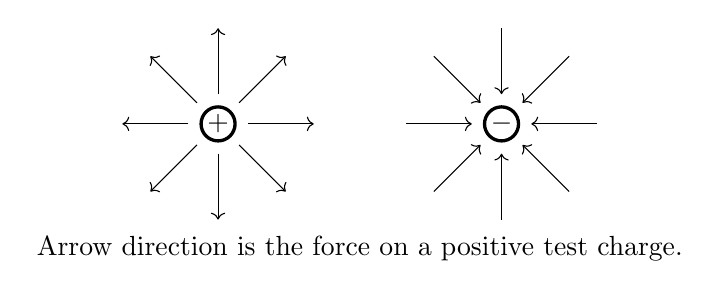
\begin{tikzpicture}[scale=.9]
\draw[very thick] (0,0) circle (.24); \node at (0,0){$+$};
\foreach \a in {0,45,...,315}{\draw[->] ({.42*cos(\a)},{.42*sin(\a)})--({1.35*cos(\a)},{1.35*sin(\a)});}
\draw[very thick] (4,0) circle (.24); \node at (4,0){$-$};
\foreach \a in {0,45,...,315}{\draw[<-] ({4+.42*cos(\a)},{.42*sin(\a)})--({4+1.35*cos(\a)},{1.35*sin(\a)});}
\node[below] at (2,-1.45){Arrow direction is the force on a positive test charge.};
\end{tikzpicture}\end{center}}
\newcommand{\coildiagram}{\begin{center}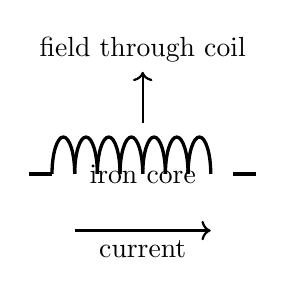
\begin{tikzpicture}[x=.72cm,y=.72cm]
\draw[very thick] (-2,0)--(-1.6,0);
\foreach \x in {-1.6,-1.2,...,1.2}{\draw[very thick] (\x,0) arc (180:0:.2 and .65);}
\draw[very thick] (1.6,0)--(2,0);
\draw[->,thick] (-1.2,-1)--(1.2,-1) node[midway,below]{current};
\draw[->,thick] (0,.9)--(0,1.8) node[above]{field through coil};
\node at (0,0){iron core};
\end{tikzpicture}\end{center}}
\newcommand{\inductiondiagram}{\begin{center}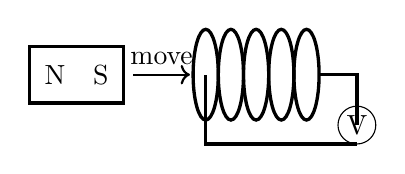
\begin{tikzpicture}[x=.8cm,y=.8cm]
\draw[very thick] (-2,-.45) rectangle (-.5,.45); \node at (-1.25,0){N\quad S};
\draw[->,thick] (-.35,0)--(.55,0) node[midway,above]{move};
\foreach \x in {.8,1.2,...,2.4}{\draw[very thick] (\x,0) ellipse (.2 and .72);}
\draw[very thick] (2.6,0)--(3.2,0)--(3.2,-.8);
\draw (3.2,-.8) circle (.3); \node at (3.2,-.8){V};
\draw[very thick] (3.2,-1.1)--(.8,-1.1)--(.8,0);
\end{tikzpicture}\end{center}}

\telosmeta{Electricity \& Magnetism}{\doctitle}{\docsubtitle}{20260726.001}
\begin{document}
\telosmasthead[\editiontag\ --- \docstrap]
\rolecard
\begin{materials}\materialslist\end{materials}
\begin{predict}\prediction\end{predict}
\diagram
\section{Investigate}
\procedure
\section{Explain from the evidence}
\explanation
\section{Change one thing}
\extension
\begin{recordbox}\end{recordbox}
\sourcefoot
\end{document}

